\section{Unsupervised Activity Representation}
\label{basics}
Here we explain the generative model which we use in order to jointly learn the activities from videos. We start with explaining the basic notation we use in the model. We denote the $t^{th}$ frame of the $i^{th}$ video as $I^i_t$ and its subtitle as $L^i_t$. Moreover, we note the extracted frame representation as $y^i_t$. We model our algorithm based on activities and the note the activity of the $t^{th}$ frame of the $i^{th}$ video as $z^i_t$. Since our model is non-parametric, number of activities are not fixed and $z^i_t \in \mathcal{N}$.

\paragraph{Frame:} Representation of each frame is computed as the occurence vector over the detected language and visual atoms. Formally, frame $y^i_t$ is represented as $y^i_t=[y^{i,l}_t,y^{i,v}_t]$ such that $k^th$ entry of the $y^{i,l}_t$ is $1$ if the frame as language atom $k$ and $0$ otherwise. $y^{i,l}_t$ is also a binary vector similarly defined over visual atoms. We consider $y^i_t$ as the observed variable and consider the underlying activity label as the hidden state $z^i_t$. A sample state is visualized in the Figure \ref{visFrame}.

\begin{figure}
  \caption{Visualziation of the representation of the Frame.}
\end{figure}

\paragraph{Activity:} We represent each activity as a Bernoulli distribution over the visual and language atoms. In other words, each frame's representation $y^i_t$ is sampled from its activity distribution as $y^i_t|z^i_t=k \sim Ber(\Theta_k)$. For the sake of clarity, we sample the $\Theta$ from its conjugate distribution \emph{Beta distribution}.

In the following sections, we exlpain how these models can be jointly learned and inferred by using the Beta Process Hidden Markov Models.
s
\subsection{Beta Process Hidden Markov Model}
For joint understanding of the time-series information, Fox et al.\cite{foxBPHMM} proposed the Beta Process Hidden Markov Models (BP-HMM) using the Indian Buffet Process\cite{ibp} of time-series sequences over features. It assumes that there exist a set of features(activities in our case) which can explain the behaviour of all time-series data (all videos in our case). Each time-series data exhibits a subset of available features. This setup is similar to Hughes et al.\cite{npActivity}. However, we differ in the choices of the underlying distributions since we based our model on semantic multi-modal information.

In our model, each video $i$ chooses a set of activities through a activity vector $\mathbf{f^i}$ such that $f^i_k$ is $1$ if $i^th$ video has activity $k$, 0 otherwise. When the feature vectors of all videos in the courpus is concatanated, it becomes an activity matrix $\mathbf{F}$ such that $i^th$ row of the $\mathbf{F}$ is the activity vector $\mathbf{f^i}$. Moreover, each feature $k$ also has an activity frequency $b_k$  and a distribution parameter $\Theta_k$. Distribution parameter $\Theta_k$ is the Bernoulli distribution as explain in the Section \ref{basics}. Moreover, its base distribution ($B_0$) is \emph{Beta random variable} since it is the conjugate of Bernoulli.
 Moreover, in this setting, the activity paremeters $\Theta_k$ and $b_k$ follow the \emph{beta process} as;
\begin{equation}
  B|B_0,\gamma,\beta \sim \text{BP}(\beta,\gamma B_o), B=\sum_{k=1}^\infty b_k \delta_{\Theta_k}
\end{equation}
where $B_0$ and the $b_k$ are determined by the underlying poisson process \cite{hbp} and the feature vector is determined as independent Bernoulli draws as $f_{k}^i \sim Ber(b_k)$. After marginilizing over the $b_k$ and $\Theta_k$, this distribution is shown to be equivalent to Indian Buffet Process \cite{bpibp}. Where videos are customers and activities are dishes in the buffet. The first video chooses a $\text{Poisson}(\gamma)$ unique dishes. The following video $i$ chooses previously sampled activity $k$ with probability $\frac{m_k}{i}$ proportional to number of videos ($m_k$) chosen the activity $k$, and it also chooses $\text{Poisson}(\frac{\gamma}{i})$ new activities. Here, $\gamma$ controls the number of active features in each video and $\beta$ controls the likelihood of the features getting shared by multiple videos.

After each video chooses a subset of activities, we model the videos as an Hidden Markov Model (HMM) over the selected videos. Each frame has the hidden state activity id($z^i_t$) and we observe the binary representation $y^i_t$. Since we model each activity as a Bernoulli distribution, the emmition probabilities follow the Bernoulli distribution as $p(y^i_t|z^i_t)=Ber(\Theta_{z^i_t})$. Following the construction of the Fox et al.\cite{foxBPHMM}, we sample the transition probabilities from a normalized Gamma distribution. For each video $i$, we sample a Gamma random variable for the transition between activity $j$ and activity $k$ if both of the activities are included by the video (if $f^i_k$ and $f^i_j$ are both $1$). After sampling these random variables, we normalize them to have proper transition probabilities. This procedure can be represented formally as
\begin{equation}
  \eta_{j,k}^i \sim Gam(\alpha+\kappa \delta_{j,k},1), \quad \pi_j^i = \frac{\eta^i_j \circ f^i}{\sum_k \eta^i_{j,k} f^i_k}
\end{equation}
Where $\kappa$ is the persistence parameter promoting self state transitions to have more coherent temporal bounderies, $\circ$ is the element-wise product and $\pi^i_j$ is the transition probabilities in video $i$ from state $j$ to all states in the form of a vector.

This model is also presented as a graphical model in Figure \ref{bphmmo}
\begin{figure}[h!]
  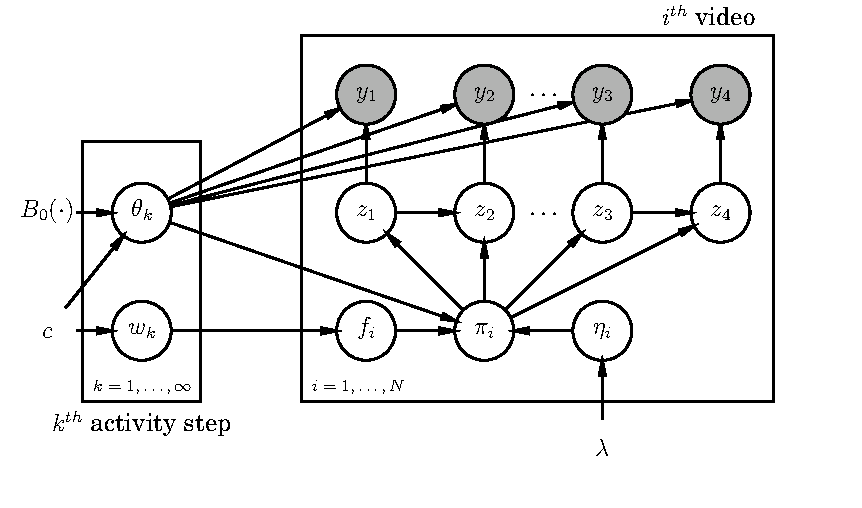
\includegraphics[width=0.5\textwidth]{plate}
  \caption{\textbf{Graphical model for BP-HMM:}Some explanation.}
  \label{bphmmo}
\end{figure}


\subsection{Gibbs sampling for BP-HMM}
We employ Markov Chain Monte Carlo (MCMC) method for learning and inference of the BP-HMM. We base our algorithms on the MCMC procedure proposed by Fox et al.\cite{foxBPHMM}. It marginilizes over blah and blah and sample blah and blah. For faster convergence, we also utilize a series of data driven samplers. Here we only discuss the proposed data driven samplers and move the details of the remainin samplers to the Supplementary Material.

\paragraph{Data-Driven Sampler1}
\paragraph{Data-Driven Sampler2}
